\chapter{日志084-A4}

\label{chap:DOC-log-084-a4}

\bb{观测到的\hyperref[chap:SCP-084]{SCP-084}相关异常事件记录}

\begin{figure}[H]
    \centering
    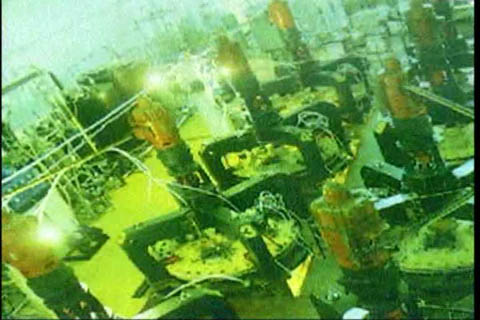
\includegraphics[width=0.5\linewidth]{images/log.084.a4.jpg}
    \caption*{B-4小队记录的图像。目标图像是一堵正在“闪烁”的墙。}
\end{figure}

\hr

关于占作用区域大部分面积的“草原”的详细观察记录。平原看上去由同一块十(10)米×十(10)米的草地无限重复所组成。草地块组合时似乎有随机“旋转”,导致草地块和地面的微小变化出现排列错误。

\hr

很少有非人类生物存在于作用区域内部。作用区域外部的动物会避开该区域,且在进入区域不久后就似乎“突然消失”了。在作用区域内观察到的动物看上去是正常的,但是行为怪异。颤抖着的动作、突然的“哆嗦”、重复的“循环”以及其他异常行为似乎暗示它们可能不是真实的动物。大多数动物似乎在3-4小时后“闪烁”并消失。

\hr

在作用区域内部难以用声音交流。在距离谈话对象五米范围内,声音交流似乎是正常的,但据报告称经常有轻微的“阻隔感”。五米之外,对象就像在非常远的地方说话,并伴有严重的回音。对象停止说话数秒后听到声音以及无人说话时传来言语的事也时有发生。

\begin{figure}[H]
    \centering
    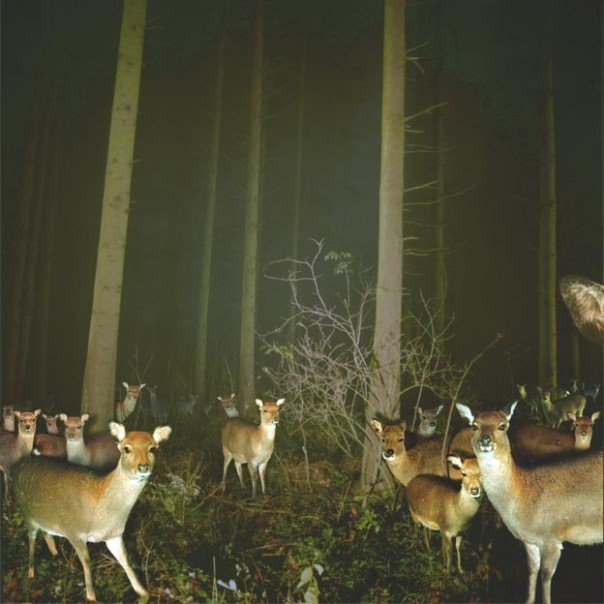
\includegraphics[width=0.5\linewidth]{images/log.084.a4.2.jpg}
    \caption*{平民拍下的图像。目标图像是一只“循环”中的鹿。}
\end{figure}

\hr

由于不能在物理层面上到达“无线电塔”,且其“广播”效应对大部分观测设备有效,无法对其进行细致观察。最简单的单筒或双筒望远镜系统看到的塔“模模糊糊”“被静止的雾包围”,而更高级的设备又会受“异常广播”影响。

\hr

天气模式和基础的日夜循环似乎都完全随机。头顶的天空会随机地在白天和夜晚、晴朗和其它天气模式间交替。太阳和云的相对位置同样随机,在不同状态之间会规律性地“闪烁”和“模糊”。

\hr

在作用区域内不可能对任何物体造成物理性的改变或损坏。挖掘、拆除和新的建设等行为会突然“变模糊”并被“重置”到之前某一个时间点的未经改变的状态。在“重置”结构中的实验者——例如身处一个洞中——会立刻被困住且被“融合”。

\hr

SCP-084周边作用区域内的人类显示出一些更加显著和容易观察的现实扭曲效应。这包括:

\begin{itemize}
\item 四肢或头部突然“模糊”,看上去以极高的速度旋转数秒。对象没有疼痛感,也常常意识不到此现象。
\item “循环”,一般表现为八(8)到二十(20)秒时间的重现。对象完成某动作(例:出门、捡起一件衣服),然后突然“定住”并“闪烁”,之后回到“循环”的初始位置重复该动作,即使这需要突然“传送”到相当长的一段距离外。罕见的情况下,对象会陷入一个永久的循环。
\item 对██████████ █████居民的观察和讯问表明在长期处于作用区域内后不再需要基础的人类需求,如食物、水和睡眠等。一些人称(他们相信)自己五(5)年不曾吃喝。一名老人同时称已自杀失败两千一百一十(2,110)次。
\item 有时人可以平安穿过固体物质。这些时段的持续时间似乎随机,开始和结束也毫无预兆。时段结束时在固体物质“内”的对象将被困住或“融合”直到这种时段再次开始。一人报告腰部以下曾困在一堵墙内两(2)年。
\item 观察到在长时间暴露下心理上的极度痛苦。辐射波的传输{[}数据删除]被长时间的暴露破坏的阻碍。处于晚期的“接收”状态的人一般在数月后“重置”。
\end{itemize}

\begin{figure}[H]
    \centering
    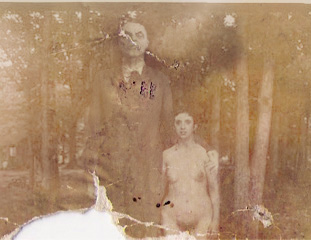
\includegraphics[width=0.5\linewidth]{images/log.084.a4.3.jpg}
    \caption*{{[}数据删除]图像}
\end{figure}

\hr

记录到的辐射波表现出一个总体上略微{[}数据删除]的循环。登记并记录这些广播的尝试因此移交给自动系统,以免再损失任何基金会人员。
